\documentclass[12pt]{article}
\usepackage[utf8]{inputenc}
\usepackage[italian]{babel}
\usepackage{makeidx}
\usepackage{graphicx}
\usepackage{listings}
\usepackage{color}
\usepackage{float}

\definecolor{dkgreen}{rgb}{0,0.6,0}
\definecolor{gray}{rgb}{0.5,0.5,0.5}
\definecolor{mauve}{rgb}{0.58,0,0.82}

\lstset{frame=tb,
  language=C,
  aboveskip=3mm,
  belowskip=3mm,
  showstringspaces=false,
  columns=flexible,
  basicstyle={\small\ttfamily},
  numbers=none,
  numberstyle=\tiny\color{gray},
  keywordstyle=\color{blue},
  commentstyle=\color{dkgreen},
  stringstyle=\color{mauve},
  breaklines=true,
  breakatwhitespace=true,
  tabsize=4
}


\graphicspath{ {./images/} }


\title{WIND - Lattice-Boltzmann Fluid Dynamics}
\author{Antonino Natale, 200705}
\date{Luglio 2020}


\begin{document}
\selectlanguage{italian}

\maketitle

\begin{abstract}
I metodi reticolari di Boltzmann, in fluidodinamica computazionale, sono un insieme di tecniche usate per la simulazione dei fluidi.
L'equazione di Boltzmann viene risolta a partire dalle equazioni di Navier-Strokes per simulare il flusso di un fluido newtoniano mediante modelli di collisione.
In questo documento, mi occuperò principalmente di questo particolare automa cellulare sfruttando un approccio volto all'efficenza e scalabilità richiesta dalla complessità computazionale dello stesso.
\end{abstract}


\tableofcontents
\newpage

\section{Introduzione}
\index{Introduzione}
\subsection{Dinamica dei fluidi}
La fluidodinamica è una branchia notoriamente difficile della fisica, dove pochissimi problemi possono essere risolti analiticamente.
Un fluido, può subire oscillazioni lineari proprio come un solido, ma a differenza di quest'ultimo può anche scorrere attorno ad ostacoli e, in molte circostanze anche ruotare vorticosamente su stesso.
Questo comportamento è intrinsecamente non lineare e difficile da comprendere in modo quantitativo.
Normalmente, descriviamo lo stato macroscopico di un fluido in termini di densità \( \rho \), e di velocità \( \vec{u} \), entrambi in funzione di posizione e tempo.
A queste funzioni seguono un insieme di equazioni differenziali parziali, chiamate \textit{equazioni di Navier-Strokes}, le quali derivano dalle leggi di Newton e da alcune assunzioni empiriche riguardo il comportamento dei fluidi.
A causa della complessità analitica delle equazioni di Navier-Strokes, nei problemi di fluidodinamica, si preferisce un approccio computazionale. Nascono quindi, i \textit{Computational Fluid Dynamics (CFD)}, ovvero metodi di discretizzazione delle equazioni di Navier-Strokes, con conseguente risoluzione numerica per date condizioni a contorno. 

\subsection{I reticoli di Boltzmann}
Nell'approccio dei reticoli di Boltzmann, discretizziamo sia spazio che tempo, affinchè siano permesse solo ed esclusivamente certe velocità vettoriali discrete.
Nel progetto, la struttura reticolare utilizzata è la \textbf{D2Q9}, dove si assume uno spazio a due dimensioni \( xy \) e nove possibili componenti vettoriali \( \vec{e} \).
Una di queste componenti è zero, mentre le altre otto descrivono una particella e i suoi possibili movimenti nelle otto direzioni adiacenti al reticolo - orizzontale, verticale e diagonale.

\begin{center}
    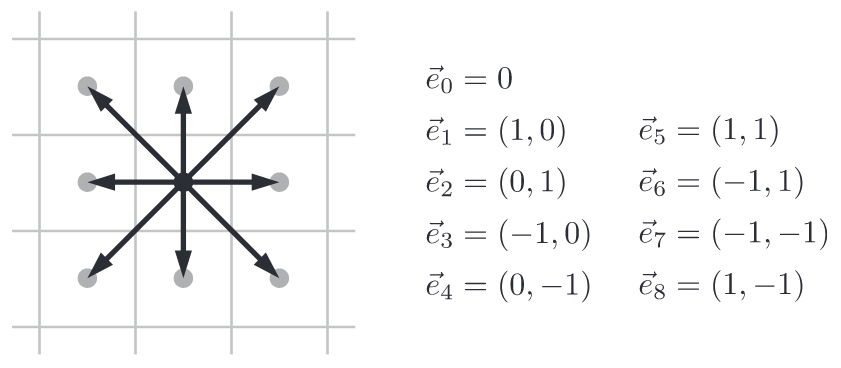
\includegraphics[scale=0.5]{1}
\end{center}


L'obiettivo è quello di associare delle probabilità \(w_i\) a questi nove vettori velocità, al fine di garantire l'accuratezza della distribuzione di Boltzmann.
Per un fluido in quiete con velocità \( \vec{u} = 0 \), la probabilità ottimale risulta essere \(\frac{4}{9}\); per uno in movimento nelle quattro direzioni cardinali è \(\frac{1}{9}\), e per le diagonali \(\frac{1}{36}\).

\begin{equation}
    w_0 = \frac{4}{9}
\end{equation}

\begin{equation}
    w_1 = w_2 = w_3 = w_4 = \frac{1}{9}
\end{equation}

\begin{equation}
    w_5 = w_6 = w_7 = w_8 = \frac{1}{36}
\end{equation}


\subsubsection{Equazione di equilibrio}
\label{sec:desc}
Nell'algoritmo dei reticoli di Boltzmann, elementi di particolare rilevanza sono le nove densità microscopiche \(n_i(x,y)\), che scorrono attraverso le nove componenti vettoriali \(\vec{e_i}_i\) di ogni reticolo.
In un dato istante di tempo, per ogni reticolo, queste nove densità possono avere valori positivi che sommati tra loro restituiscono la densità macroscopica \(\rho\), e i componenti \(x\) e \(y\) della vettore velocità macroscopica \(\vec{u}\).
I risultati di queste due variabili costituiscono le componenti essenziali per l'equazione di equilibrio termico:

\begin{equation}
\label{eqn:eq}
    n^{eq}_i = \rho w_i [1 + 3 \vec{e}_i \cdot \vec{u} + \frac{9}{2}(\vec{e}_i \cdot \vec{u})^2 - \frac{3}{2}|\vec{u}|^2] 
\end{equation}

Il primo passo è quindi quello di calcolare, per ogni step della simulazione, la (\ref{eqn:eq}) ad ogni singolo reticolo che compone il fluido.
Applicando quindi:

\begin{equation}
\label{eqn:update}
    n^{new}_i = n^{old}_i + \omega (n^{eq}_i - n^{old}_i)
\end{equation}

Lasciamo che le nove densità microscopiche si avvicinino, poco per volta, all'equilibrio termico \(T\).
Dove \(\omega\) è un valore scalare che indica la \textit{viscosità} del fluido, ovvero quanto più tempo le collisioni impiegano nel processo di equilibrio - può assumere valori da \(0\) a \(2\).



\subsubsection{Algoritmo}
\label{sec:alg}

Per ogni step della simulazione si applicano i seguenti passi:
\begin{enumerate}
    \item \textbf{Collisione.} Per ogni reticolo:
    \begin{enumerate}
        \item Dalle nove densità microscopiche \(n_i\) si costruiscono \(\rho\) e \(\vec{u}\);
        \item Si applica la (\ref{eqn:eq}) per calcolare l'equilibrio termico \(T\);
        \item Si aggiornano le nove densità microscopiche in accordo con l'equazione (\ref{eqn:update}). 
    \end{enumerate}
    \item \textbf{Scorrimento.} Per ogni reticolo, si scorrono le densità \(n_i\) che lo compongono nei rispettivi reticoli adiacenti, copiandone l'appropriato valore;
    \item \textbf{Rimbalzo.} Per ogni barriera - condizione a contorno - si inverte lo scorrere delle densità \(n_i\) alterandone il vettore \(\vec{u}\).
\end{enumerate}


\newpage
\section{Calcolo Parallelo}
\subsection{Message Passing Interface}

MPI è uno standard di comunicazione tra nodi appartenenti ad un cluster di computer che eseguono un programma parallelo.
Lo scopo nel progetto è di accelerare, mediante parallelizzazione su più nodi, l'esecuzione dell'algoritmo dei reticoli di Boltzmann, al fine di avere una simulazione interattiva e in tempo reale dello scorrimento di un fluido newtoniano attraverso degli ostacoli inseriti dall'utente.
Realizzare ciò, ha richiesto la considerazione di un nuovo approccio che fosse efficente, in termini di prestazioni, e scalabile, ovvero, utilizzabile in un cluster più complesso costruito su più nodi, anche remoti.
Prima di descrivere il metodo utilizzato è doveroso introdurre due concetti fondamentali di MPI.


\subsubsection{Window Object e Memoria condivisa}
\label{sec:mpi1}
I nodi che esistono all'interno di uno stesso dispositivo fisico sono in grado di interfacciarsi tra loro mediante tecniche di memoria condivisa. Ossia, richiedono al sistema operativo un'area di memoria visibile ad entrambi i processi, nella quale inserire direttamente informazioni e dati senza ricorrere all'utilizzo delle routine \verb|MPI_Send/MPI_Recv|.
MPI, allora, introduce una nuova entità, chiamata \verb|Window| con lo scopo di gestire zone di memoria condivisa.
In particolare, nel progetto, ho utilizzato la funzione:

\begin{lstlisting}
    MPI_Win_allocate_shared (
        unit_size * sizeof(struct unit), 
        sizeof(struct unit), 
        MPI_INFO_NULL, 
        MPI_COMM_LOCAL, 
        &units, 
        &MPI_LOCAL_WINDOW
    );
\end{lstlisting}

Il risultato è analogo alla funzione \verb|MPI_Scatter()|, ossia, l'area di memoria viene partizionata per singolo nodo.
La differenza è che ciò permette di allocare zone di memoria adiacenti e condivise per ogni singolo nodo all'interno di un dato gruppo \verb|MPI_COMM_LOCAL|.

\begin{figure}
    \centering
    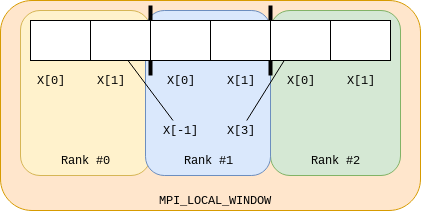
\includegraphics[scale=0.75]{3}
    \caption{Area di memoria condivisa all'interno di un Window Object}
    \label{fig:winobj}
\end{figure}




\subsubsection{Comunicatori}
\label{sec:mpi2}
Un comunicatore è un oggetto che descrive un gruppo di nodi all'interno di un cluster.
Per questo progetto si è reso necessario suddividere i nodi al fine creare gruppi di comunicatori locali che interagissero tra loro e condividessero la stesso oggetto \verb|Window|.
Il motivo, è principalmente prestazionale; i gruppi sono suddivisi secondo il criterio \verb|MPI_COMM_TYPE_SHARED|, ovvero gruppi di nodi, facenti parte dello stesso dispositivo fisico, che possono creare un area di memoria condivisa.

\begin{lstlisting}
    MPI_Comm_split_type (
        MPI_COMM_WORLD, 
        MPI_COMM_TYPE_SHARED, 
        world_rank,
        MPI_INFO_NULL, 
        &MPI_COMM_LOCAL
    );
\end{lstlisting}

Ciò permette ad ogni singolo nodo all'interno di ogni gruppo \verb|MPI_COMM_LOCAL| di condividere, in modo diretto e veloce, i propri dati sulla simulazione in corso.


\begin{figure}
    \centering
    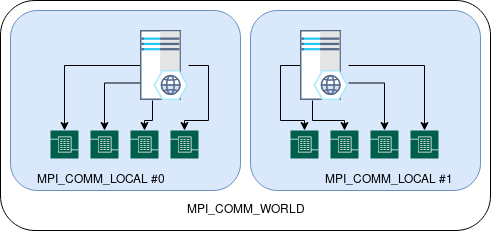
\includegraphics[scale=0.5]{2}
    \caption{Topologia dei nodi}
    \label{fig:comm}
\end{figure}





\subsection{Parallelizzazione e Ghost Cells}
Sfruttando i concetti di \ref{sec:mpi1} e \ref{sec:mpi2}, ho deciso di suddividere i nodi per gruppi \verb|MPI_COMM_LOCAL| dal gruppo globale più grande \verb|MPI_COMM_WORLD| ed assegnare loro un \verb|local_rank| e un \verb|world_rank| di riferimento.
Ad ogni \verb|MPI_COMM_LOCAL| ho allocato una \verb|MPI_LOCAL_WINDOW| di dimensioni pari ai reticoli che ogni nodo deve gestire.
Infine, l'algoritmo si sviluppa principalmente in tre fasi:

\begin{enumerate}
    \item \textbf{Collisione.} Per ogni nodo locale, eseguo i calcoli di \ref{sec:alg}
    \item \textbf{Scorrimento Locale.} Per ogni nodo locale applico lo scorrimento descritto in \ref{sec:alg} accedendo alle aree condivise di memoria degli altri nodi locali appartenenti allo stesso gruppo \verb|MPI_COMM_LOCAL|
    \item \textbf{Scorrimento Globale.} Per ogni nodo locale adiacente ad un altro \verb|MPI_COMM_LOCAL| esterno, utilizzo le routine \verb|MPI_Send/MPI_Recv| al fine di ottenere le \textit{Ghost Cells} ed applicare a quest'ultime lo scorrimento dei reticoli.
\end{enumerate}

\subsubsection{Vantaggi}
I vantaggi risiedono principalmente nel numero ridotto di chiamate ad \verb|MPI_Send/MPI_Recv|, con conseguente diminuzione drastica dei tempi di esecuzione, necessari al fine di ottenere una simulazione rapida e in tempo reale.



\begin{figure}
    \centering
    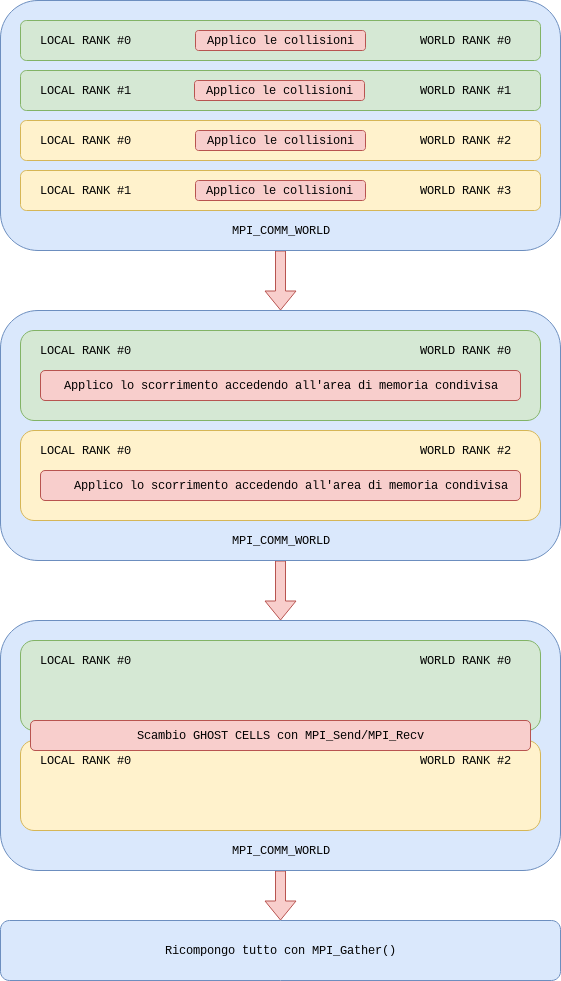
\includegraphics[scale=0.55]{4}
    \caption{Algoritmo in parallelo}
    \label{fig:parallel_algorithm}
\end{figure}




\newpage
\section{Progetto}
Infine, veniamo al codice. Tutto ciò che è stato accennato nelle prime sezioni è trascritto in C++ all'interno del progetto, con l'ausilio di \verb|OpenMPI| e \verb|Allegro|.


\subsection{Variabili}

\subsubsection{Units}
Matrice di locale di reticoli di Boltzmann. Viene assegnata ad ogni nodo presente in \verb|MPI_COMM_WORLD| ed è definita come \verb|struct unit* units;|

\subsubsection{Frame}
Matrice globale di reticoli di Boltzmann. Viene allocata solo ed esclusivamente dal nodo primario di \verb|MPI_COMM_WORLD|, ossia con \verb|world_rank = 0|. Il suo scopo è puramente di disegno e raccolta delle computazioni dei singoli nodi ed è definita come \verb|struct unit* frame;|

\subsubsection{Ghost Cells}
Matrice mono-dimensionale che descrive la riga, qualora vi fosse, superiore o inferiore del reticolo locale \verb|units|. Sono due e sono definiti come \verb|struct unit* up_units| e \verb|struct unit* bottom_units|.

\subsubsection{Velocità e viscosità fluido}
Entità che descrivono la velocità \(\vec{u}\) e la viscosità \(\omega\) del fluido, vedi \ref{sec:desc}.
Sono definite come \verb|v2d flow_speed;| e \verb|double flow_viscosity;|

\subsubsection{Booleane di controllo}
Permettono di interagire con l'esecuzione della simulazione, sono: \verb|running|, \verb|paused|, \verb|resetting|.


\subsubsection{MPI\_COMM\_LOCAL}
Comunicatore creato a partire dal gruppo principale \verb|MPI_COMM_WORLD| che contiene nodi facenti parte dello stesso dispositivo fisico.

\begin{lstlisting}
    MPI_Comm_split_type (
        MPI_COMM_WORLD, 
        MPI_COMM_TYPE_SHARED, 
        world_rank, 
        MPI_INFO_NULL, 
        &MPI_COMM_LOCAL
    );
\end{lstlisting}


\subsubsection{MPI\_LOCAL\_WINDOW}
Window Object che descrive l'area di memoria condivisa all'interno di ogni singolo \verb|MPI_COMM_LOCAL|

\begin{lstlisting}
    MPI_Win_allocate_shared (
        unit_size * sizeof(struct unit), 
        sizeof(struct unit), 
        MPI_INFO_NULL, 
        MPI_COMM_LOCAL, 
        &units, 
        &MPI_LOCAL_WINDOW
    );
\end{lstlisting}


\subsubsection{Ranks e num\_procs}
Entità di tipo intero che identificano informazioni riguardo al gruppo globale/locale di appartenenza.

\begin{lstlisting}
    MPI_Comm_rank(MPI_COMM_WORLD, &world_rank);
    MPI_Comm_size(MPI_COMM_WORLD, &world_num_procs);
    
    MPI_Comm_rank(MPI_COMM_LOCAL, &local_rank);
    MPI_Comm_size(MPI_COMM_LOCAL, &local_num_procs);
\end{lstlisting}


\subsection{Strutture Dati}
Sono presenti diversi tipi di \verb|MPI_DataType|. Il loro scopo è quello di ottimizzare il processamento dei dati da parte delle routine di MPI.



\subsubsection{Vettore}
L'entita che descrive un vettore bidimensionale è definita come \verb|struct v2d| e contiene:
\begin{itemize}
    \item Componente \(X\)
    \item Componente \(Y\)
\end{itemize}

\begin{lstlisting}

    MPI_Datatype v2d_types[] = { MPI_DOUBLE, MPI_DOUBLE };
    MPI_Aint v2d_offsets[]   = { 0, sizeof(double) };
    int v2d_blocks[]         = { 1, 1 };

    MPI_Type_create_struct (
        2, 
        v2d_blocks, 
        v2d_offsets, 
        v2d_types, 
        &MPI_TYPE_V2D
    );
    
    MPI_Type_commit(&MPI_TYPE_V2D);

\end{lstlisting}

\subsubsection{Reticolo}
L'entità che descrive il reticolo di Boltzmann è definita come \verb|struct unit| e contiene:
\begin{itemize}
    \item Tipo di unita: Fluido, Barriera
    \item Le nove densità microscopiche \(n_i\)
    \item Densità macroscopica \(\rho\)
    \item Vettore velocità \(\vec{u}\)
    \item Intensità del vortice limitrofo
\end{itemize}

\begin{lstlisting}

    MPI_Datatype unit_types[] =
        { MPI_DOUBLE, MPI_CXX_BOOL, MPI_TYPE_V2D, MPI_DOUBLE, MPI_DOUBLE };
        
    MPI_Aint unit_offsets[] = {
        offsetof(unit, n),
        offsetof(unit, barrier),
        offsetof(unit, u),
        offsetof(unit, rho),
        offsetof(unit, curl),
    };

    int unit_blocks[] = { 9, 1, 1, 1, 1 };

    MPI_Type_create_struct (
        5, 
        unit_blocks, 
        unit_offsets, 
        unit_types, 
        &MPI_TYPE_UNIT
    );
    
    MPI_Type_commit(&MPI_TYPE_UNIT);
    
\end{lstlisting}



\subsection{Avvio}
All'avvio, il nodo primario globale, ossia con \verb|world_rank = 0| alloca le strutture di cui necessita per il disegno e inizializza \verb|Allegro|, istanzia una finestra ed effettua il polling degli eventi, gestendo grafica e input utente.
In seguito, ogni nodo, dopo aver istanziato le entità di MPI, da inizio all'esecuzione dell'algoritmo descritto in \ref{sec:alg}.
Il fluido, inizialmente è in uno stato di quiete, ovvero di equilibrio termico. Non appena l'utente disegna, alterando la morfologia delle condizioni a contorno, avviene la destabilizzazione del fluido stesso, portando a tale risultato:


\newpage
\begin{figure}
    \centering
    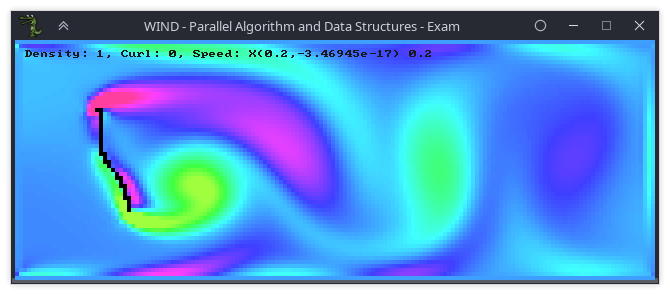
\includegraphics[scale=0.75]{5}
    \caption{Avvio e disegno di una barriera}
    \label{fig:startup}
\end{figure}



Come si può notare dalla figura (\ref{fig:startup}), la posizione e rotazione della barriera al centro crea una turbolenza con il susseguirsi di vortici instabili di colore verde e fucsia.



\subsection{Istruzioni}
L'utente può interagire con la simulazione attraverso Mouse e Tastiera con i seguenti comandi.

\subsubsection{Tastiera}
\begin{itemize}
    \item \textbf{R}: Sospende/Riprende la simulazione
    \item \textbf{C}: Cancella tutte la barriere
    \item \textbf{I}: Mostra topologia dei nodi globali
    \item \textbf{U}: Mostra topologia dei nodi locali
    \item \textbf{1 .. 5}: Cambia modalità di visualizzazione: 
        \begin{enumerate}
            \item Vortici
            \item Densità
            \item Velocità totale
            \item Velocità X
            \item Velocità Y
        \end{enumerate}
    \item \textbf{NumPad}: Cambia direzione del fluido.
\end{itemize}

\subsubsection{Mouse}
L'utente può disegnare le barriere sullo schermo cliccando con il tasto sinistro del mouse.


\subsection{Benchmarks}
I test sono eseguiti su: \\

\begin{left}
    \verb|Linux 5.4.44-1-LTS|
\end{left}

\begin{left}
    \verb|Intel(R) Core(TM) i3-4160 CPU @ 3.60GHz (Dual Core)|
\end{left}


\begin{center}
    \centering
    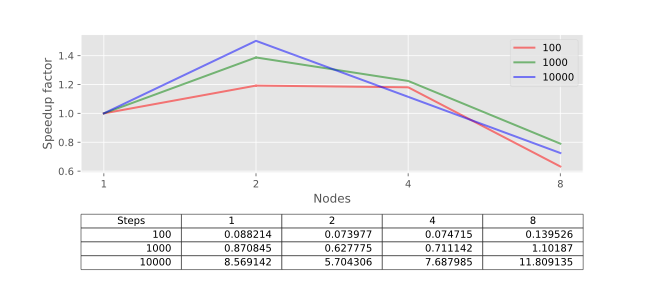
\includegraphics[scale=0.75]{bench}
    \caption{Benchmark e Speedup factor}
    \label{fig:bench}
\end{center}




\subsection{Screenshots}



\begin{center}
    \centering
    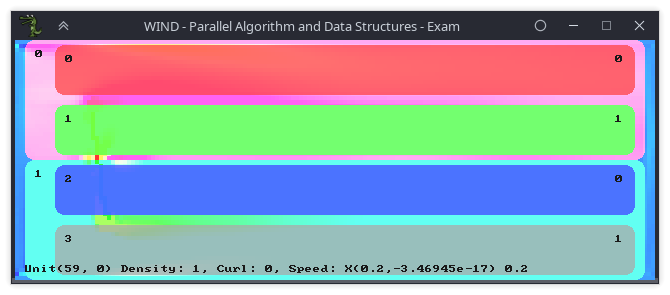
\includegraphics[scale=0.75]{7}
    \caption{Esempio di Topologia. A sinistra il rank globale, a destra quello locale}
    \label{fig:screen0}
\end{center}

Questo è un esempio di topologia dove sono presenti due \verb|MPI_COMM_LOCAL| e quattro nodi distruibuiti: due per il primo gruppo, due per il secondo.



\begin{center}
    \centering
    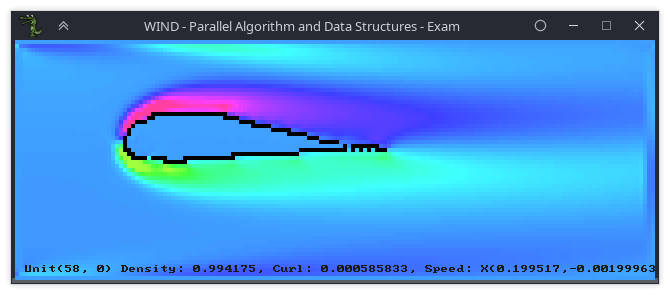
\includegraphics[scale=0.75]{8}
    \caption{Piano a profilo aerodinamico}
    \label{fig:screen2}
\end{center}

\begin{center}
    \centering
    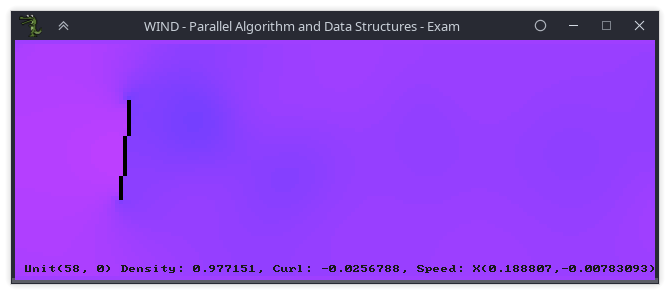
\includegraphics[scale=0.75]{9}
    \caption{Densità fluido}
    \label{fig:screen3}
\end{center}

\begin{center}
    \centering
    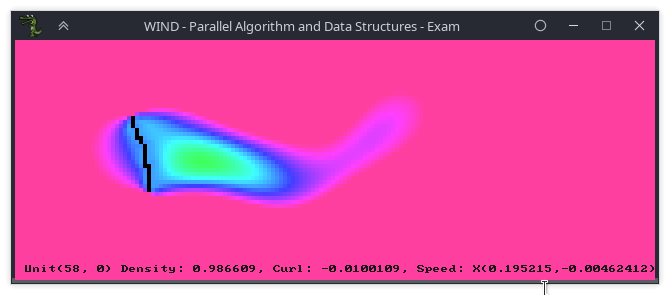
\includegraphics[scale=0.75]{10}
    \caption{Velocità \(\vec{u}\) totale}
    \label{fig:screen4}
\end{center}

\end{document}
